\graphicspath{{content/chapters/literature_review/datasets/figures}}

\section{Datasets}
\label{sec:datasets}

There are 4 \gls{vqa} datasets that will be explored and discussed in this section. As the strengths and scopes of each one are discussed, a final dataset will be discussed which goes a step beyond \gls{vqa}.

\subsection{SHAPES}
\label{subsec:shapes_dataset}

\begin{figure}[htbp]
    \centering
    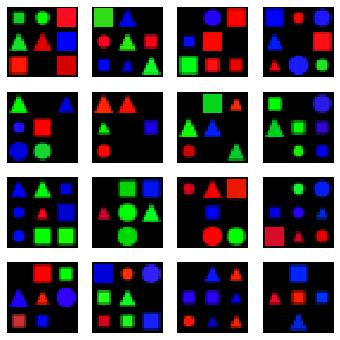
\includegraphics[width=.35\textwidth,keepaspectratio]{shapes_example_images}
    \captionsource(Example SHAPES entries){Example images from the SHAPES dataset. \label{fig:shapes_example_images}}{\url{https://paperswithcode.com/dataset/shapes-1}}
\end{figure}

The SHAPES dataset is a \gls{vqa} dataset introduced by \citeauthor{andreas_deep_2016} \cite{andreas_deep_2016} consisting of synthetic images designed to test the layout construction of compositional neural models.
Each image-question pair consists of a simple image with 9 possible locations for objects and a number of visible shapes in each image.
These shapes are simple uniform shapes (triangles, squares, or circles) with only a difference in color  (red, green, or blue) to distinguish them (see Figure~\ref{fig:shapes_example_images}).
The questions on the other hand are complex with each question containing up to 4 different object attributes, types, or relationships.
The questions found in the dataset can be deliberately false (such as \texttt{Is a red shape blue?} or \texttt{Is the red square a triangle?}) or valid questions (such as \texttt{Is the red object left of a blue triangle a square?}).

\subsection{VQA}
\label{subsec:vqa_dataset}

\begin{figure}[htbp]
    \centering
    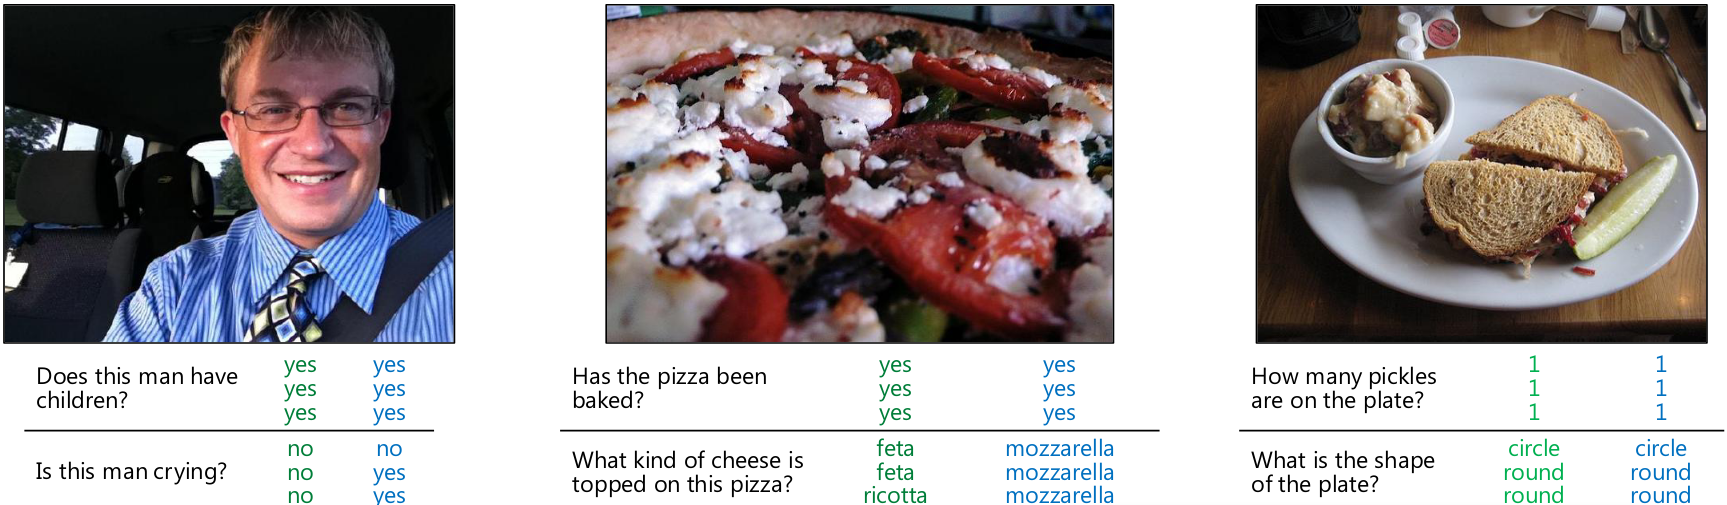
\includegraphics[width=\textwidth,keepaspectratio]{vqa_questions_answers}
    \captionsource(Example \acrshort{vqa} entries){Example images from the \acrshort{vqa} dataset with a question per image and answers. Green answers are valid answers for the given image while blue answers would be valid without the image. Only the green answers are used throughout. \label{fig:vqa_questions_answers}}{\citeauthor{agrawal_vqa_2016}\cite{agrawal_vqa_2016}}
\end{figure}

The VQA dataset \cite{agrawal_vqa_2016} is a natural image dataset composed of 204,721 images, 1,105,904 questions, and 10 acceptable ground truth answers per question.
The images are taken from the COCO image dataset \cite{lin_microsoft_2015} real-life objects, scenarios, and entities, while the questions and answers are supplied by human annotators.
All questions are open-ended, with an array of possble answers to select from and a subset of answers which are possible/correct (See Figure~\ref{fig:vqa_questions_answers} for example image-question pairs with answers).

\subsection{CLEVR}
\label{subsec:clevr_dataset}

\begin{figure}[htbp]
    \centering
    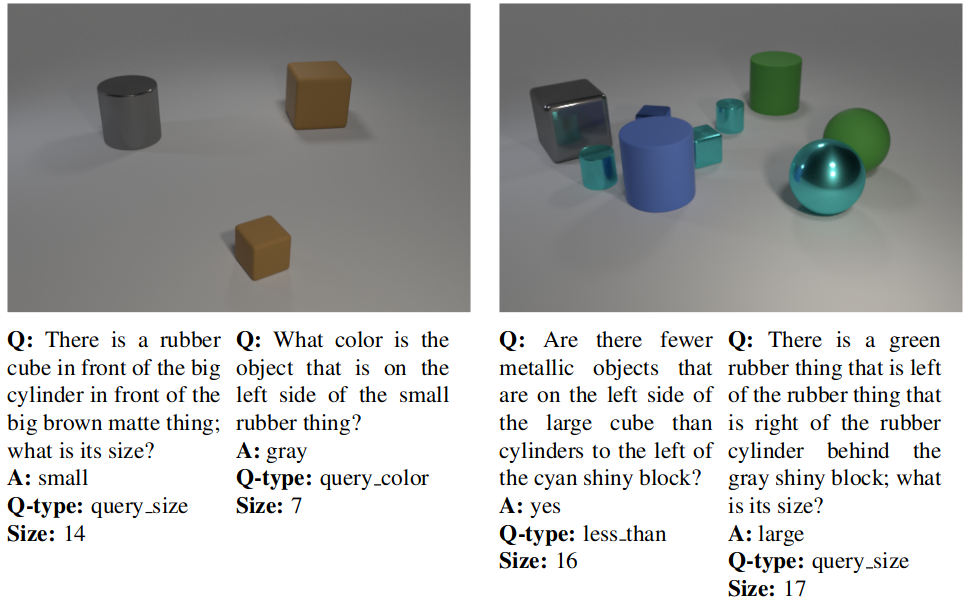
\includegraphics[width=\textwidth,keepaspectratio]{clevr_questions_answers}
    \captionsource(Example CLEVR entries){Example images from the CLEVR dataset with a question per image and the correct answer. Additionally, there's also the type of question included (such as classifying the size or colour) and the size of the datasets included expert layout/program. \label{fig:clevr_questions_answers}}{\citeauthor{johnson_clevr_2016}\cite{johnson_clevr_2016}}
\end{figure}

The CLEVR dataset \cite{johnson_clevr_2016} is a \gls{vqa} dataset designed to test and benchmark compositional \gls{vqa} models.
Similar to the \hyperref[subsec:shapes_dataset]{SHAPES} dataset, each image is a blank scene with any number of 3d shapes which can differ in shape, colour, size, and material (being either shiny metal, or matte rubber).

Questions vary in the type of answer expected (such as counting, yes/no, object attributes), and are diverse in structure, length, query types used through and relationship queries (see Figure~\ref{fig:clevr_questions_answers}).
In total, CLEVR contains 100,000 images and 864,968 questions, with a single correct answer being given per question.

\subsection{GQA}
\label{subsec:gqa_dataset}

\begin{figure}[htbp]
    \centering
    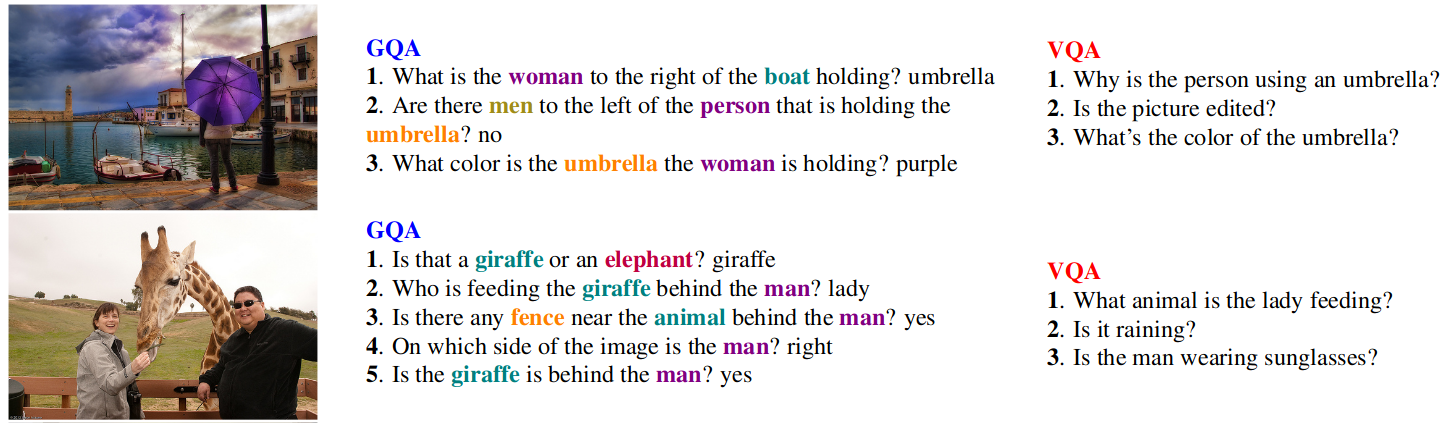
\includegraphics[width=\textwidth,keepaspectratio]{gqa_vqa_questions_comparison}
    \captionsource(Example GQA questions){Comparison of questions from both GQA (left) and \gls{vqa} (right) datasets for the same image. The GQA questions feature greater emphasis on object relations and compositionality than the \gls{vqa} questions are which are comparatively vague or ambiguous. \label{fig:gqa_and_vqa_questions_compared}}{\citeauthor{hudson_gqa_2019}\cite{hudson_gqa_2019}}
\end{figure}

The \gls{gqa} dataset was introduced by \citeauthor{hudson_gqa_2019}\cite{hudson_gqa_2019} as a collection of highly compositional questions to better train compositional \gls{vqa} models.
The dataset contains over 110,000 images --- sourced from various image datasets --- and over 22,000,000 questions.
\todo[inline]{Elaborate further?}

Alongside each image is a scene-graph which describes the objects in the image, object relations, and image location details.
Each question in the training set describes a program in the form of semantic steps which --- if executed by a training model --- would lead to a greater probability of predicting the correct answer.
These steps mimic how a person would apply reasoning to a question to provide an answer to it and should therefore train a model how to perform such reasoning.

\subsection{VCR}
\label{subsec:vcr_dataset}

The VCR dataset \cite{zellers_recognition_2019} was introduced alongside the formalisation of the \gls{vcr} task as the first dataset of the kind.
The images in the dataset are largely frames from movies or clips, and are chosen because of the inherent context supplied by the movies that's required to understand the images.
Because of this, each question in the dataset is about something present within context that cannot be immediately recognised by simple object detection and will thus require additional cognition to answer.
The questions, answers, and rationales, also make use of bounding boxes to identify each person/object of interest, and uses their box names when referring to them (see Figure~\ref{fig:vcr_question_answer} for an example of how these are used).
Aside from answering each question, there is also a further task of providing rationale behind the given answer.
In this subtask, the model would have to produce its reasoning for predicting the initial answer by predicting the correct rationale for the correct answer.
There is only one correct answer and one correct rationale per-question.
There are 3 modes of question-answering available by the dataset as broken down below:

\begin{itemize}\label{list:vcr_task_types}
    \item (Q \rightarrow A): Predict the correct answer for a given image and question.
    \item (QA \rightarrow R): Predict the correct rationale for the given answer to a given question and image.
    \item (Q \rightarrow AR): Using only the image and question, predict both the correct answer and correct rationale.
\end{itemize}

\begin{figure}[htbp]
    \centering
    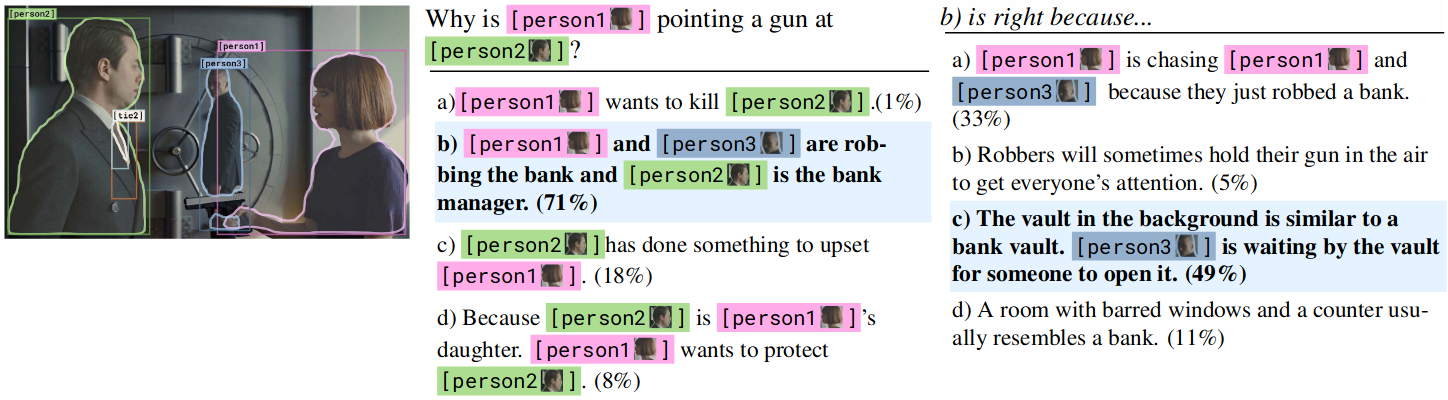
\includegraphics[width=\textwidth,keepaspectratio]{vcr_question_answer}
    \captionsource(Example \acrshort{vcr} entry){Example \acrshort{vcr} task from the \acrshort{vcr} dataset. The text shows how each object in the image is highlighted by the provided bounding box metadata. \label{fig:vcr_question_answer}}{\citeauthor{zellers_recognition_2019}\cite{zellers_recognition_2019}}
\end{figure}

In total, there are 99,904 images, 264,720 questions, 1,058,880 answers, and 1,058,880 rationale.
Each image in the dataset comes with many question files, each containing a question about the image with one correct answer and one correct rationale per-question.
A further 3 incorrect answers and 3 incorrect rationale are included with the correct ones, which are correct answers or rationale to one other question in the dataset (in other words, each answer/rationale is correct at least once across all questions in the dataset).
Each question file (outside of the test fold) specifies the correct answers for the question, and the 'correctness' of each answer.
% Not all information about the file is discussed (such as the ids of each question relative to the image or fold it belongs to).
Each image is accompanied with a metadata json file containing the dimensions of the image, the class names of the objects present (eg. person, car, dog, etc), and the bounding boxes and polygons identifying each object in the image.
All bounding boxes and polygons were generated using the Detectron object detection system\cite{Detectron2018}.

\subsection{VisDial}
\label{subsec:visdial_dataset}

\begin{figure}[htbp]
    \centering
    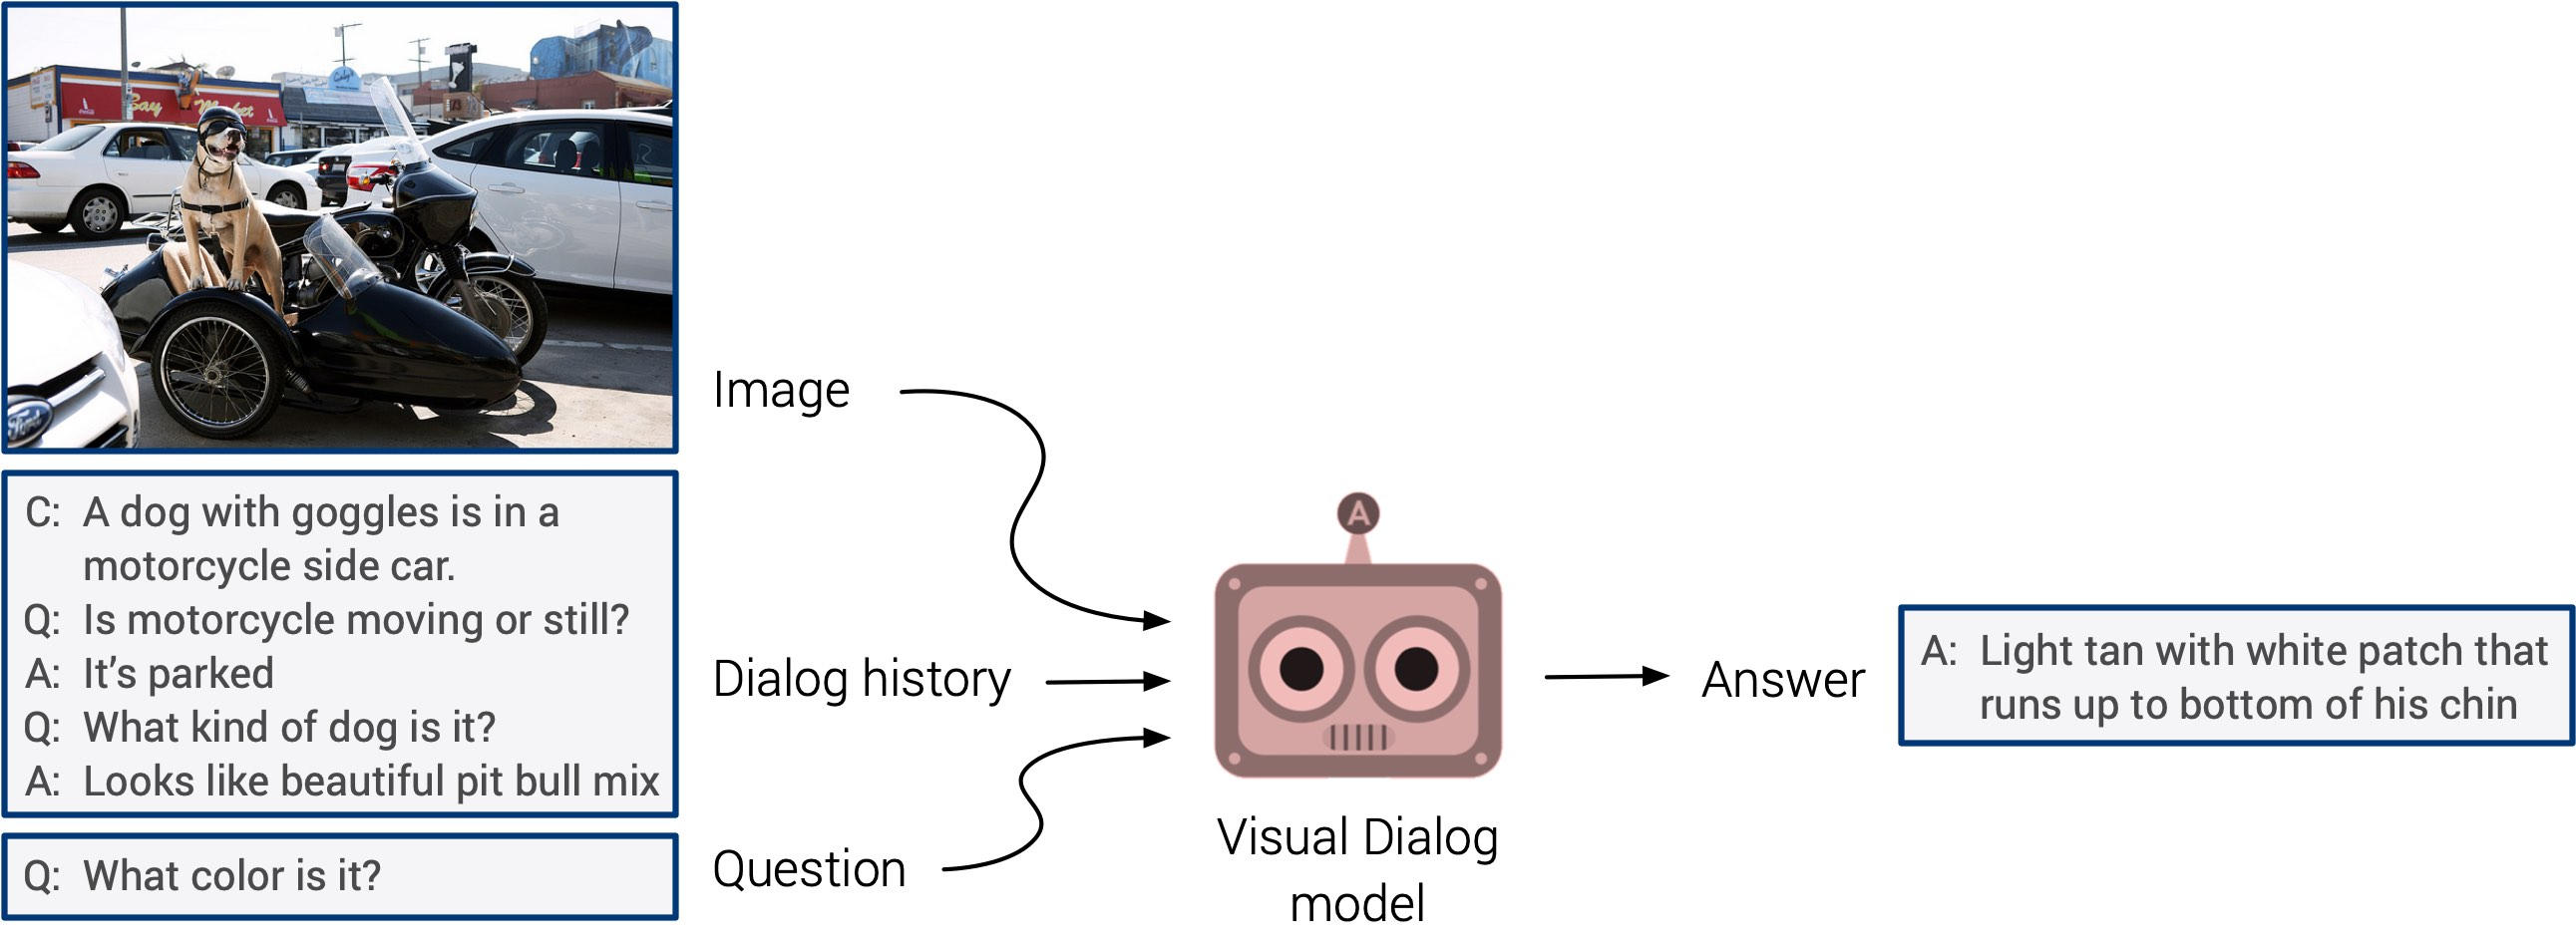
\includegraphics[width=\textwidth,keepaspectratio]{visdial_dataset_overview}
    \captionsource(Example VisDial entry){Example \gls{vd} task from the VisDial dataset. The image is supplied with a caption, a model predicts answers to the questions for that image, and the model must maintain context for each following question using the dialogue history. \label{fig:visdial_question_answer}}{\url{https://visualdialog.org}}
\end{figure}

The VisDial dataset --- published by \citeauthor{das_visual_2019} \cite{das_visual_2019} --- formalises a new visual task known as \glsfirst{vd}.
Where \gls{vqa} and \gls{vcr} both focus on an image with a single question and answer, \gls{vd} extends this by posing multiple questions per image to be answered sequentially, building a natural-flowing dialogue in the process.
The dataset is composed of roughly 140,000 total \gls{vd} entries where each entry contains one image sourced from the COCO dataset\cite{lin_microsoft_2015}, one caption describing the image, and ten rounds of questions and answers.
The questions in the image were created without access to the image, only the caption.
Aside from this, subsequent questions also build upon the new context derived from answers to previous questions such as asking for more details about the previous answer.
This causes the questions to flow like a natural dialogue between two persons, where the model is the only subject to know what's present in the picture.
Another benefit to this approach is that it reduces the \gls{vpb} typically found in other visual datasets, where questions would focus only on visible subjects and therefore have easily-predictable answers.
Evaluation on these \gls{vd} tasks is performed using a custom evaluation protocol published alongside the dataset; given the image, the image caption, the dialog history up until the question to be answered, the question to be answered, and the top candidate answers (where N = 100), the model must produce a sorted list of the candidate answers for the given question.
Its performance is then evaluated by comparing the rank of the human response in the sorted list, checking if the response is in the top-k responses (\it{recall@k}), and the reciprocal rank of the human response among all other answers.
Finally, the authors also publish a set of 3 encoders that show how to encode a \gls{vd} task in a machine model.
These encoders either embed the data in vector space and generate a joint embedding, use a sequence of \glspl{rnn} with attention-over-history to the question-relevant history, or simply store the data in memory and perform lookup when generating a final context vector.
\todo[inline]{The \gls{vd} models analysed later attempt to solve a problem unique to this task and perhaps \gls{vcr} too known as the 'visual coreference problem'. This involves more than one pronoun or word referring to the same thing. Expand it or build upon this shared feature of both datasets.}
